%!xelatex = 'xelatex --halt-on-error %O %S'

\documentclass{buaaemp}
\begin{document}

% 标题,作者
\emptitle{氦氖激光器的模式分析}
\empauthor{智朝晖}{钱建强}

% 奇数页页眉 % 请在这里写出第一作者以及论文题目
\fancyhead[CO]{{\footnotesize 智朝晖: 氦氖激光器的模式分析}}


%%%%%%%%%%%%%%%%%%%%%%%%%%%%%%%%%%%%%%%%%%%%%%%%%%%%%%%%%%%%%%%%
% 关键词 摘要 首页脚注
%%%%%%%%关键词
\Keyword{He--Ne激光器, FP扫描干涉仪, 模式分析, 谱线宽度,纵模间隔}
\twocolumn[
\begin{@twocolumnfalse}
\maketitle

%%%%%%%%摘要
\begin{empAbstract}
激光作为受激辐射效应的直接应用,在理论和实验的研究中均有重要的意义。本实验利用FP扫描干涉仪对He--Ne激光器进行了模式分析,观察并记录各种参数变化对频谱波形的影响,并观察分析多模激光器的模谱,记下波形,测量计算出纵模间隔。同时测量每个纵模的谱线宽度,将示波器上的波形放大,测出每个尖峰的半宽度,利用类似计算纵模间隔的方法计算谱线宽度,最后得到激光增益曲线宽度。
\end{empAbstract}

%%%%%%%%首页角注,依次为实验时间、报告时间、学号、email
\empfirstfoot{2022-10-20}{2022-10-20}{20377365}{20377365@buaa.edu.cn}
\end{@twocolumnfalse}
]
%%%%%%%%!首页角注可能与正文重叠,请通过调整正文中第一页的\enlargethispage{-3.3cm}位置手动校准正文底部位置:
%%%%%%%%%%%%%%%%%%%%%%%%%%%%%%%%%%%%%%%%%%%%%%%%%%%%%%%%%%%%%%%%
%  正文由此开始
\wuhao 
%  分栏开始

\section{理~~论}
	1917年前后,爱因斯坦(A. Einstein)首先在旧量子论的框架内描述了原子的受激辐射\cite{einstein1917quantentheorie}。人们猜想这一现象可用于加强光场,这便是激光,即\textit{受激辐射光放大}(Light Amplification by
	Stimulated Emission of Radiation, LASER or laser)之起源。
	
	1957年,贝尔实验室(Bell Labs)的查尔斯·汤斯(C. H. Townes)和阿瑟·肖洛(A. Schawlow)在利用氖光灯照射稀土晶体时,首先观察到了晶体产生的激光\cite{schawlow1958infrared}。事实上,在此之前,\textit{微波放大}(Microwave Amplification by Stimulated Emission of Radiation, MASER or~maser)已经实现,并对激光的设计带来了很大的启发\cite{townes1999laser}。
	
	在波长 \SI{632.8}{\nm} 可见光区工作的He--Ne气体激光器同样由贝尔实验室于1962年开发,这是目前应用最为广泛的激光器之一\cite{white1962continuous}。
 
\subsection{激光}
	当原子处于激发态$E_2$时,如果恰好有能量为$(E_2-E_1)$的光子入射,在入射光子的影响下,原子会发出一个同样的光子而跃迁到低能级$E_1$上去,这便是受激辐射(stimulated emission)。这里,\textit{“同样”}意味着受激辐射发出的光子和外来光子的频率、相位、传播方向以及偏振状态全同。

\newpage
	如今,利用薛定谔方程及含时微扰的办法,可以更为严谨地导出受激辐射现象;参见 \cite{griffiths2016introduction}, \textbf{单个}原子在外场下受激辐射与吸收光子的概率实际上是等同的。然而,对于处在平衡态的大量原子而言,相应能态上的粒子数遵循统计分布;事实上,粒子数目随能态增高而指数地减少,即:\vspace{-2ex}
	\begin{equation}
		E_2 > E_1,\quad N_2 \ll N_1
	\end{equation}
	
	因此,对一个由大量原子组成的纯粹的二能级系统而言,虽然存在受激辐射,但其发生的概率远小于吸收,不能产生激光。由此可见,产生激光的前提和关键在于粒子数反转,所以需要用有\textbf{激励能源}和\textbf{增益介质},即设法使$N_2 > N_1$并维持如此。更细致的分析还应考虑统计分布导致的权重;一般来说,要求:
	\begin{equation}
		\frac{N_2}{g_2} > \frac{N_1}{g_1}
	\end{equation}
	$g_{1,2}$即为统计权重。

\subsection{激光器}
	本实验所用的He--Ne激光器中,实际产生激光(发生受激辐射)的是Ne原子,He原子则起\textit{传递能量}的作用,以实现粒子数反转;具体流程如图 \ref{fig:HeNeLevel} 所示。
	\begin{figure}[!h]
	\centering
	\vspace{-1.2\baselineskip}
	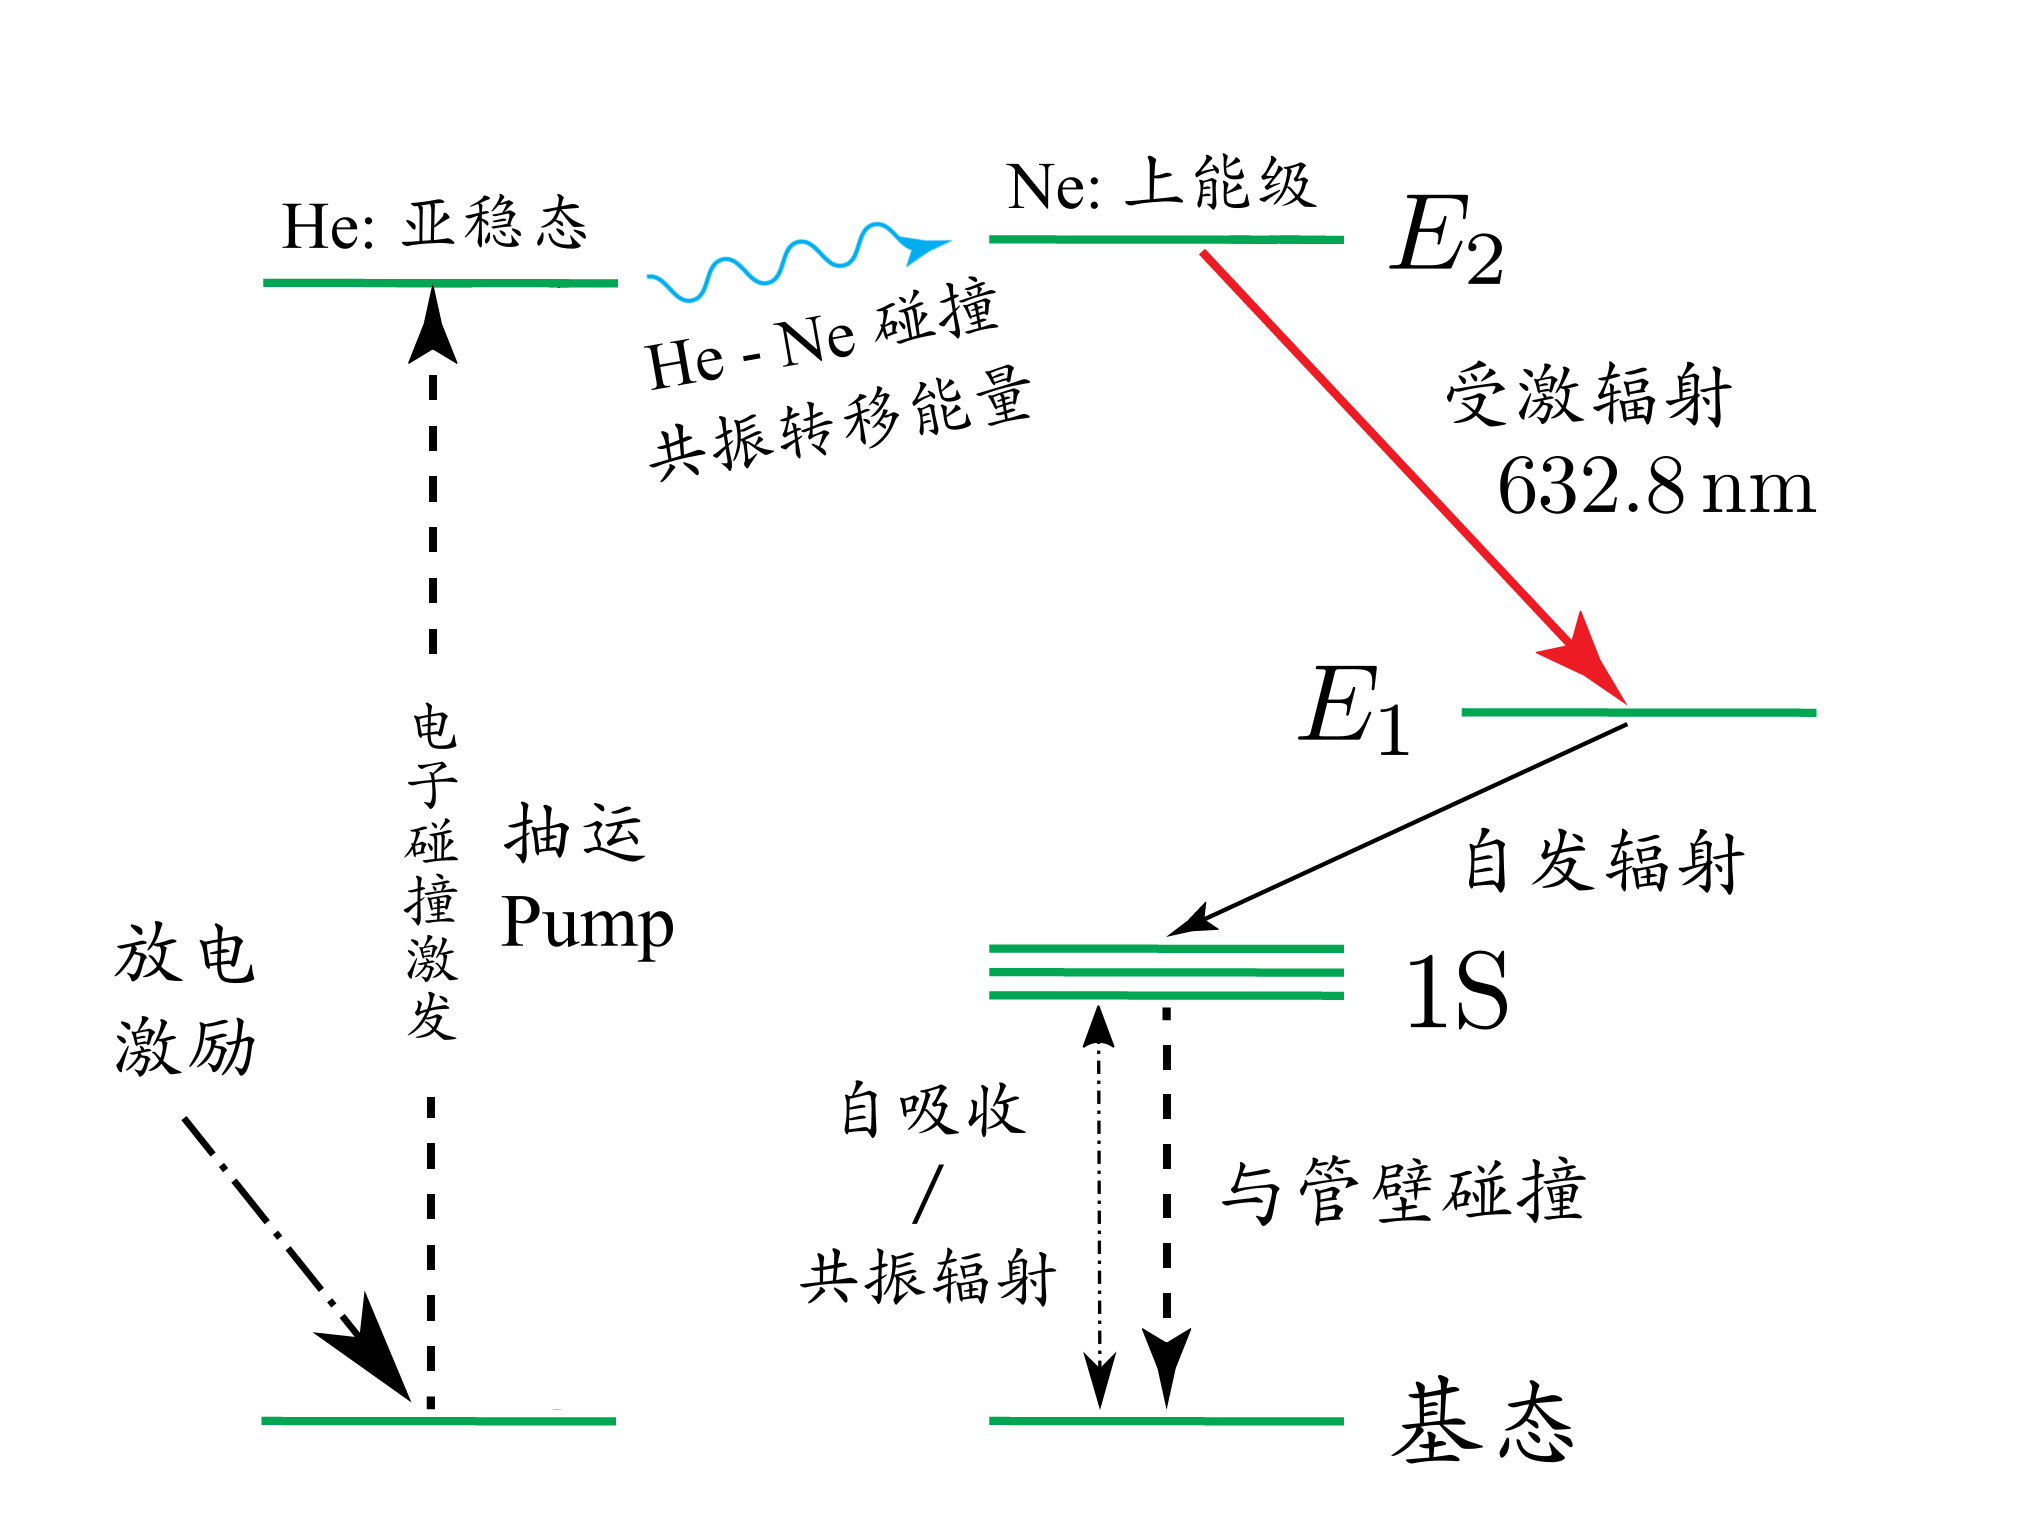
\includegraphics[width=.8\linewidth]{image/HeNeLaserLevel.png}
	\caption[\textup{He--Ne}激光原理]{%
		\textup{He--Ne}激光发生过程的能级示意图\footnote{%
			图像据网络资源修改得到:\par
			\noindent%\fontsize{9pt}{\parskip}%
			\url{https://en.wikipedia.org/wiki/File:HeNe_Laser_Levels.png}%
		},参考 \cite{javan1961population}. \\[1ex]
		注:示意图中的能级间隔不全按照比例,但相对高低与实际一致;\\
		\textup{He}的亚稳态($2^1\rm{S}_0$)与\textup{Ne}的上能级($3\rm{S}_2$)实际十分接近,图中夸大了两者的差距。\\
		另外,图中仅体现了 \SI{632.8}{\nm} 的受激辐射。
		\vspace{1ex}
	}
	\label{fig:HeNeLevel}
	\end{figure}
	
	这里应当注意,图 \ref{fig:HeNeLevel} 中的中间能态$1\rm{S}$中存在亚稳态,同时$1\rm{S}$跃迁至基态发出的共振辐射容易被别的基态Ne原子吸收,即发生\textit{自吸收}过程\cite{javan1961population};这相当于延长了$1\rm{S}$态的寿命,导致处在该低能态的粒子数目较多,不利于维持粒子数反转。相应的解决办法是:设法增大气体容器的管壁面积,使处在$1\rm{S}$态的Ne原子与管壁碰撞回到基态。因此,本实验中的气体放电在\textbf{毛细管}中进行。
	
	此外,He--Ne混合气体的受激辐射频率并非只有 \SI{632.8}{\nm}; 事实上,最早实现的He--Ne气体激光器正是工作在红外波段(\SI{1.15}{\um},参见 \cite{javan1961population})。同时,单个谱线还存在一定的展宽,这也应当加以考虑。综上所述,有必要使用光学\textbf{谐振腔}进行选频、增强;本实验中使用的光学谐振腔结构如图 \ref{fig:gasTube} 所示。
	\begin{figure}[!h]
	\centering
	\vspace{-.5\baselineskip}
	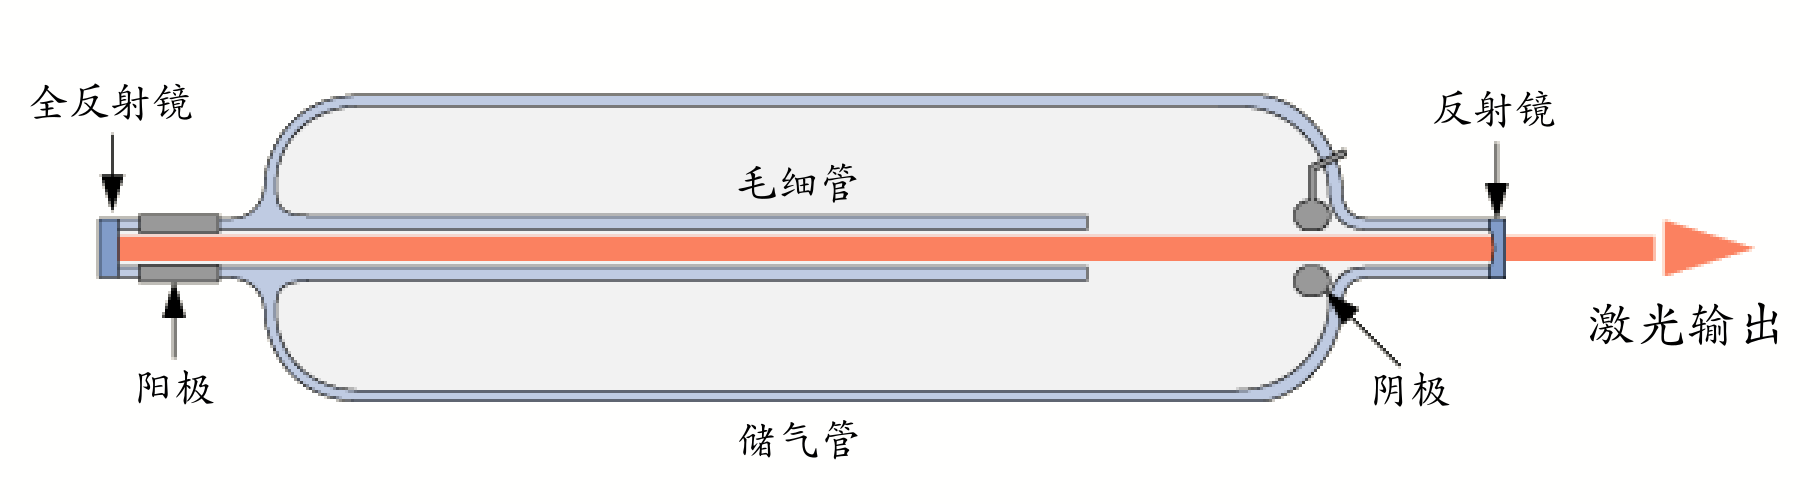
\includegraphics[width=.9\linewidth]{image/gasTube.png}
	\caption[\textup{He--Ne}激光管结构]{%
		\textup{He--Ne}激光管结构示意图\footnote{%
			图像据网络资源修改得到:\par
			\noindent%\fontsize{9pt}{\parskip}%
			\url{https://en.wikipedia.org/wiki/File:Hene-1.png}%
		},本实验中毛细管直径$d\sim\SI{1.25}{\mm}$. \vspace{1ex}
	}
	\label{fig:gasTube}
	\end{figure}


激光形成持续稳定的增长振荡的条件是光在谐振腔中往返一周的光程差是波长的整数倍:
\begin{equation}
    2 \mu L=q \lambda
\end{equation}
其中$\mu$是折射率(对气体$\mu$=1),$L$是腔长,每一个 $q$对应着纵向一种稳定的电磁场分布(纵模),其频率以及纵模间距为:
\begin{equation}
    \nu_1=q \frac{c}{2 \mu L} \\
    \Delta \nu_{\Delta q=1}=\frac{c}{2 \mu L} \approx \frac{c}{2L}
\end{equation}

其增益曲线如图\ref{fig:mode}所示:
\begin{figure}
    \centering
    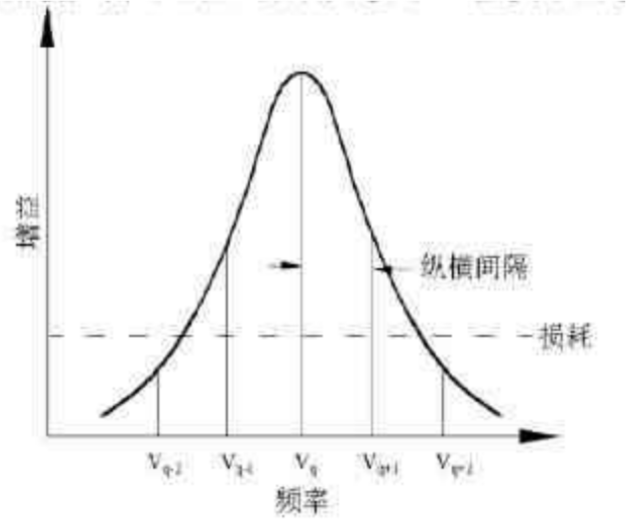
\includegraphics[width=.9\linewidth]{image/fre.png}
    \caption{纵模和纵模间距}
    \label{fig:mode}
\end{figure}
同时还有跳模、增益饱和和稳频等现象。

\subsection{FP扫描干涉仪}
FP扫描干涉仪是一种分辨率很高的光谱分析仪器,光线正入射时的相干干涉条件为:
\begin{equation}
    4 \eta L=m \lambda
\end{equation}
固定一块反射镜,另一块做周期振动,干涉仪便对允许透射的光波波长进行扫描,当$L$改变$\lambda /4$时,干涉仪改变一个干涉级,此时两干涉级之间允许透射的频率差为自由光谱范围:
\begin{equation}
    \elta \mu_F =\frac{c}{4 \eta F}
\end{equation}
\section{实验数据}
本实验观察并记录各种参数变化对频谱波形的影响,并观察分析多模激光器的模谱,记下波形,测量计算出纵模间隔。同时测量每个纵模的谱线宽度,将示波器上的波形放大,测出每个尖峰的半宽度,利用类似计算纵模间隔的方法计算谱线宽度,最后得到激光增益曲线宽度。如表\ref{tab:2},\ref{tab:3}所示:
\begin{table}[]
    \centering
    \begin{tabular}{ccc}
    \hline
         & $\delta t_M / \mu s$ & $ \delta t / \mu s$ \\ \hline
第一组 & 400                                              & 1440                                          \\ \hline
第二组 & 420                                              & 1440                                          \\ \hline
第三组 & 410                                              & 1430                                          \\ \hline
第四组 & 410                                              & 1440                                          \\ \hline
第五组 & 410                                              & 1440     \\ \hline
    \end{tabular}
    \caption{ 自由光谱范围和纵模频率间隔对应的$\delta t_M\ \delta t $}
    \label{tab:1}
\end{table}


\begin{table}[]
\centering
\begin{tabular}{lll}
\hline
    & $\delta t / \mu s$& $\Delta t /\mu s $\\ \hline
第一组 & 552                                           & 34                                            \\ \hline
第二组 & 539                                           & 33                                            \\ \hline
第三组 & 546                                           & 33          \\
\hline

\end{tabular}
\caption{半峰宽对应的$\delta t\ \Delta t $}
\label{tab:2}
\end{table}

\begin{table}[]
    \centering
    \begin{tabular}{cccc}
    \hline
         &  $\delta t_1$ &$\delta t_2$ & $\delta t_3$ \\ \hline
        $\delta t / \mu s$ & 980 & 980 & 970 \\ \hline
    \end{tabular}
    \caption{增益曲线宽度对应的$ \delta t $}
    \label{tab:3}
\end{table}

\section{实验结果与分析}
同时通过观察锯齿波信号发生器的多个参数对波形的影响,定性描述其功能为:
\begin{itemize}
    \item \textbf{光放大}\ 谱线的增益强度随着光放大而放大
    \item \textbf{直流偏置}\ 是信号发生漂移
    \item \textbf{前后沿}\ 调证锯齿波的斜率
    \item \textbf{幅度}\ 影响峰的数量
    \item \textbf{频率}\ 影响锯齿波的频率,使得扫描谱线增多
\end{itemize}
利用上述实验数据,计算实验结果得:
自由光谱范围:0.546ms
纵模间隔为:$\delta \nu_q=1.1406 GHz$
故平均半峰宽度:$4\times \frac{\sum \Delta_i}{3 \times 0.456}=0.244GHz $
平均激光增益区间:$4\times \frac{\sum d_i}{3 \times 0.456}=1.2967GHz $

\section{思考题}
\begin{itemize}
    \item 模式特点为纵模,相邻纵模频率间隔相等,对应同一组纵模。 
    \item 这是因为提高电压幅度,使得干涉仪腔长的变化也增大,可以透过的透射光的频率范围也增大。输出的模式没有增加。
    \item 锯齿波扫描信号作为X输入相当于时间分量,然后将干涉信号输出作为Y分量输入就可以得到频谱结构。
    \item 这是跳模现象,刚点燃时墙内温度升高放电管热膨胀,使得放电管两端反射镜片距离加大,当一段时间过后温度稳定距离不变时输出频谱稳定。
\end{itemize}


\section{结~~论}
本实验观察并记录各种参数变化对频谱波形的影响,并观察分析多模激光器的模谱,记下波形,测量计算出纵模间隔$\delta \nu_q=1.1406 GHz$。同时测量每个纵模的谱线宽度,将示波器上的波形放大,测出每个尖峰的半宽度0.244GHz,利用类似计算纵模间隔的方法计算谱线宽度,最后得到激光增益曲线宽度1.2967GHz。


%%%%%%%%%%%%%%%%%%%%%%%%%%%%%%%%%%%%%%%%%%%%%%%%%%%%%%%%%%%%%%%%
%  参考文献
%%%%%%%%%%%%%%%%%%%%%%%%%%%%%%%%%%%%%%%%%%%%%%%%%%%%%%%%%%%%%%%%
%  参考文献按GB/T 7714-2015《文后参考文献著录规则》的要求著录. 
%  参考文献在正文中的引用方法:\cite{bib文件条目的第一行}

\renewcommand\refname{\heiti\wuhao\centerline{参考文献}\global\def\refname{参考文献}}
\vskip 12pt

\let\OLDthebibliography\thebibliography
\renewcommand\thebibliography[1]{
  \OLDthebibliography{#1}
  \setlength{\parskip}{0pt}
  \setlength{\itemsep}{0pt plus 0.3ex}
}

{
\renewcommand{\baselinestretch}{0.9}
\liuhao
\bibliographystyle{gbt7714-numerical}
\bibliography{./TempExample}
}


\end{document}
